\chapter{Machine translation}
\label{ch:mt}
   
\section{Introduction}

%\mad{I wonder about providing some example to pull people in. Maybe something ``astoninshingly good''?} - yes, added.


Machine translation describes the task of automatically mapping a text from one human language to another.  Once considered one of the hardest problems in language technology, machine translation has seen huge advances over the past decades, and now -- for some pairs of languages, and  for some purposes -- it can be astonishingly good.   For example, a randomly chosen sentence \REF{frenchjob} from the Francophone discussion forum on Reddit (r/france) is translated instantly, fluently, and accurately \REF{englishjob} by Google Translate.  The use of the word \exword{holidays} to translate \exword{vacances} `vacation' is perhaps more British than American, but otherwise the translation is perfect:


\ea \label{frenchjob} \exsent{Pour le moment j'h\'esite \`a accepter le job parce que la position (junior) est moins bien pay\'ee que ma position actuelle d'enseignant, avec bien entendu beaucoup moins de vacances que ce que j'ai actuellement etc.}

\ex \label{englishjob} At the moment I hesitate to accept the job because the position (junior) is less well paid than my current teaching position, with of course much less holidays than what I currently have etc.

\z 


This chapter explores why and how machine translation has been so successful, and what challenges still remain.

If you are a monolingual Anglophone in an English-dominant society, you may not see a strong need for translation because you are privileged to speak an international \keyword{lingua franca} (language of trade and scholarship).  But many people around the world  speak a different language at work/school versus at home; with different members of their family; or when they travel an hour away from home.  In multilingual contexts such as the European Union, translation is needed for essentially all trade, travel, and governance.  Translation is a daily necessity for much of the world's population, and machines can make it more accessible.

Before explaining how machine translation works, it is useful to define the concept and
introduce some terms.
\keywordAs{Translation}{translation} is the process of moving text or speech from one
human language to another, while preserving the intended message.  (We'll discuss what that really means below.) We call the message's original language  the \keyword{source language} and the language that it's translated into the \keyword{target language}.
We say that two words, one from the source language,  one from the target language, are
\keyword{translation
  equivalents} if they convey the same meaning in context. The same idea applies to pairs of phrases and
sentences.

\REF{over:confident} illustrates some difficulties that can arise if you are not
careful to check whether a translation is saying the right thing (some found on the subreddit r/Engrish, some taken from  \mediatitle{Atlas Obscura}.\footnote{``Why menu translations go terribly wrong,'' 24 January 2018, by Emily Monaco})  Some of these translations were probably generated by machines, others by humans with incomplete knowledge of both languages.
If you are ever asked to put up a sign or write a menu in a language
that you do not fully understand, 
remember these examples and get the content checked!

\ea \label{over:confident} \ea \label{paris} \emph{Sign in a Paris hotel:} Please leave your values at the front desk
\ex \label{battle} \emph{Sign on a Japanese subway:} Do not pick pocket, Do not molester, Do not drug, Do not drunk and disorderly, Do not smoking, Do not battle
 \ex \label{beefl} \emph{Menu at a Russian restaurant:} Beef language with fungus sauce
 \ex \label{mouthbags} \emph{Menu at a German restaurant:} Mouth bags % Maultaschen - similar to ravioli or dumplings
 \ex  \label{cigarette} \emph{Menu at a Turkish restaurant:} Cigarette pie
 \ex \label{grass} \emph{Sign on grass in China:} Do not disturb, tiny grass is dreaming
  \ex \label{octopus} \emph{Sign at a subway station in Hong Kong:}  Please present your Octopus
  \z 
  \z 




Let's explore what went wrong here.  \REF{paris} is just a poor word choice: \exword{Valuables} is the word that the translator was searching for, and \exword{values} is unintentionally funny. % The French word \exword{valeurs} means \exword{values} and the French phrase \exword{valeurs familiales} is used in much the same way as  \exword{family values} is in English.

\REF{battle} involves confusion about grammatical categories: \exword{Do not} combines with verbs or verb phrases in English, but here it is combined with nouns (\exword{do not molester}), adjectives (\exword{do not drunk and disorderly}), and gerunds (\exword{do not smoking}).  \exword{Do not battle} is syntactically coherent, since \exword{battle} can be a verb as well as a noun, but \exword{battle} is an unusual way to describe a two-person altercation on the subway.

The next three examples \REF{beefl}--\REF{cigarette}, from menus, illustrate why culinary translation is particularly difficult.  Names for food are culturally specific and somewhat idiomatic; should they be translated literally, or elaborated for an unfamiliar audience?  What food words should be translated in the first place, versus just left in the original language?  Many food words originally enter English as \keyword{borrowings} (also known as \keyword{loan words}) from other languages (\exword{spaghetti, sushi, quesadilla}); upscale menus for  Anglophone diners are full of more recent and lesser-known loan words (\exword{ballotine, moussaka, gochujang}), which diners may look up online under the table to keep up the pretense of being cosmopolitan foodies well-versed in such vocabulary.

The \exword{language} in \REF{beefl} really means \exword{tongue}.  These two concepts are denoted by the same word in Russian.  In English, the two words are related (you use your \exword{tongue} to speak a \exword{language}) and overlap in meaning (as in \exword{mother tongue}) -- but the overlap is incomplete, because \exword{language} cannot describe a body part.   This example illustrates \keyword{polysemy} (when a word has multiple distinct but related meanings), and how a word's degree of polysemy can vary across languages.

\exword{Mouth bags} \REF{mouthbags} is an overly literal translation of German \exword{Maultaschen} `dumplings' --   small \exword{bags} of dough-wrapped filling  which go in your \exword{mouth}.   The meaning of this compound word becomes opaque and unpleasant in English,  because the word \exword{bags} is rarely used for foods, and because the relationship between the two words in the compound -- \exword{mouth} and \exword{bags} -- is not clear.  

Stepping back, a \keyword{compound} is a word made from two words (here, two nouns), with the relationship between these words supplied by the context and our background knowledge about the referent of (the thing described by) each word.  A \exword{chocolate cake}  has chocolate in it; a \exword{birthday cake} is eaten on someone's birthday; a \exword{skillet cake} is baked in a skillet. If we don't have enough background knowledge to supply this relation between the two nouns (\exword{mouth bags}), then we have to imagine one, and we may end up befuddled.  \exword{Cigarette pie} \REF{cigarette} is also a direct translation of a compound; in Turkish, it describes a long, slender pastry.  But if we don't know that \exword{cigarette} describes the shape of the pie, we may imagine that it describes an ingredient, which is less appetizing.

The final two unusual translations illustrate the challenge of translating cultural knowledge in tandem with language.  The Chinese sign \REF{grass} essentially tells people to \exword{keep off the grass}; but it uses a Chinese convention of anthropomorphizing inanimate objects and presenting directives in a cutesy, non-threatening manner.  The sign from Hong Kong \REF{octopus} seems to fantastically assume that every person has an octopus just as they have a nose and a mobile phone; but it makes sense when you understand that Hong Kong's widely-used subway/debit card is called an Octopus card.  Both of these signs may be literally translated quite well, but the informational effect on the reader is lost without cultural context.


We chose the examples in \REF{over:confident} because we hope that they are amusing. 
But in other settings, translation errors can 
have serious consequences. This happened when a 
young  patient named Willie Ramirez was brought into a Florida hospital's emergency room in a coma \citep{harsham:84}.
His
 mother and girlfriend, speaking in Spanish,
talked to the English-speaking emergency room staff.
They used the word
\exword{intoxicado}, which can mean several things, including `nauseous'.
Because the emergency room staff were not professional interpreters, they thought
that \exword{intoxicado} must mean the same as the English \exword{intoxicated} and treated
him on the assumption that he was under the
influence of drugs or alcohol. Linguistically speaking, they took \exword{intoxicado} as a \keyword{cognate}, like Spanish \exword{chocolate}, identical to the the English; but it was in fact a \keyword{false friend}, like Spanish \exword{realizar}, which does not mean `to realize' but instead means `achieve'.

%\mad{Should we point ahead to chapter 8 and mention that we're going to focus on the technology for now?} - I added a note about our recurring focus on ethics -LG.
As a result of this misunderstanding, the patient was eventually diagnosed with a brain aneurysm and
became quadriplegic. This case is infamous, because it led to a lawsuit, and drew attention to the principle that
hospitals, courts and other institutions that work with the public
should plan for the needs of a multilingual population and provide the translation and interpretation services 
that are needed.
Evoking our recurring focus on ethics, this is an issue of basic fairness, public safety, and perhaps also civil rights.  

\section{Applications of translation} \label{translateneeds}


In  information retrieval, the user can be thought of as
having an \keyword{information need} (Section~\ref{sec:information-need}). In the same way, a 
potential user of translation technology
can be thought of as having a \keyword{translation need}. 
%
%\mad{Merged little paragraphs}
Before we get into automatic translation, though, let's first explore the  needs served by human translators and interpreters.  Among human professionals, a \exword{translator} is someone who deals with text, while an \exword{interpreter} deals with speech.  

% If you have taken comparative literature classes at high school or college, you will have encountered translations into English of foreign language poetry and novels. A publisher who wants to make a new English version of a novel by Jos\'e Saramago has a translation need. This need is far beyond the capabilities of any present day automatic system, because for this purpose, a good translation needs to be a literary work in its own right. As well as getting across the content, it must capture the ``feel'' of the original writing. The only way to do this is to employ a human translator who has excellent literary skills in both English and Portuguese. Because there are so many English-speaking readers in the world, and the author is a Nobel prize winner, the publisher can expect a good return on investment in expert help. Nobody would expect a machine-generated translation to be good enough for this purpose, although it would be cheap.

%Another quite demanding translation need is that of a scholar needing to understand an academic paper written in a foreign language. Here, the scholar does not care much about the ``feel'' of the article, but will want to be sure about the arguments that are being made, the conclusions that are being drawn, and the evidence that is being used to support these conclusions. To do this well, even if the paper is in your native language, you need to have some training in the relevant academic field or fields. Academic papers are designed to be read by informed experts, so if the paper is on linguistics, what you are looking for  is a translator who is expert enough in linguistics to be able to understand and  accurately translate the arguments in the text. A translator who is a specialist in translating business documents will almost certainly struggle to make a useful translation of a  linguistics paper. We should not expect a machine translation system to be any better at meeting this specialized need.



%In chapters~\ref{ch:writers-aids} and ~\ref{ch:searching}, we described technology that supports the everyday scholarly activities of information gathering and writing. Each one of you already knows a lot about these activities. The role of the computer is to help out with the aspects of the process that it does well, and keep out of the way when the human writer knows better.  Translation is a bit different, because it is usually done by trained experts rather than the general public. Professional translators sometimes worry that machines are going to take over their role, or that  free web-based services will lead to big changes in the market for their skills. These worries are reasonable, since all knowledge workers will need to adapt as technology changes, but the reality is that professional translators are still going to be needed in future.  Unless you have had an internship with a translation company, you probably do not know as much about the market for translation as you do about the activities of writing and information gathering.  In this chapter, as well as explaining some of the technology, we will go into detail about the real-world needs for translation and the changes that are resulting from the easy availability of free online translation.

%From this perspective, literary translations are  interesting to think about when we are trying to understand the process of translation,  but are not the first place to look for practically important uses of translation technology.  For that, we need to focus on more everyday translation needs.

Among (human) interpreters, a \keyword{simultaneous interpreter} listens to speech in a source language, and speaks the same message in the target  language with only seconds' delay.  These professionals are not only fluent in both languages, but also have trained their working memory and executive functioning to listen and speak at the same time, a similar mental task to sight-reading music.   At the United Nations, diplomats wear earpieces to hear  spoken proceedings simultaneously interpreted into their own language in real time.  A \keyword{consecutive interpreter} listens to speech in a source language, takes notes, and then produces the speech in the target language  after the original source-language turn is complete.  Consecutive interpreters handle diplomatic speeches, meetings, and court cases. 
%\mad{I like learning about all these kinds of interpreters: what overarching points do we want readers to learn?} - I added a sentence at the end of this paragraph clarifying that.


A \keyword{whisper  interpreter} might accompany a diplomat to a social occasion and offer a whispered paraphrase of what people are saying, so that the diplomat can follow along politely.   A \keyword{phone interpreter} provides consecutive interpretation over the phone, for example when a doctor must provide emergency medical care to a patient in a different language, and there is no in-person interpreter on site.  Finally, a \keyword{medical interpreter} (who may work in person or over the phone) is specifically trained in medicine and ethics to provide services in a \keyword{safety-critical} context -- hopefully preventing fiascos like the one caused by the misunderstanding of \exword{intoxicado}.  Medical interpreters also have to consider the  educational background and cultural assumptions of the people  they serve; one medical interpreter \citep{Haffner:1992}  had to clarify to a patient that her fallopian tubes, once ``tied'', could not be easily untied like shoelaces.  
These different types of interpreters illustrate the diverse translation needs that arise in spoken situations.

In the rest of this chapter, we focus on translating rather than interpreting because computers deal primarily with language as text rather than speech.
All (human) translators do basically the same thing: Given a document written in a source language, they produce a corresponding document in the target language.  Different translators  specialize in  the translation of literary, technical, legal, political, historical, or medical documents, requiring rich content knowledge alongside linguistic ability.  Human translators may not write a translation from scratch, but may instead work to edit, check, and improve a draft produced by a machine, in a process called \keyword{post-editing} --  indeed \citep{Green-etal:2013}, they may find it faster and more enjoyable to work this way.

Recalling from \chapref{ch:call} that people find it easier to comprehend than to produce in their L2, both interpreters and translators may prefer to  use their L2 as the source language and their L1 as the target language.  In the context of machine translation, though, it can be equally easy to go in either direction.  

So far, we have introduced some of the translation and interpreting needs serviced by human professionals.  But there are countless other translation needs, requiring varying levels of confidence and correctness.  For each one listed here,  please consider whether you would trust a free online tool, or whether -- even considering the time and expense --  you would want to pay a human to corroborate it.   If you were to hire a human, would any bilingual person be sufficient or would you want someone with particular content knowledge?

\begin{itemize}

\item You are an award-winning Senegalese filmmaker who wants to release your Wolof-language film with English subtitles for an Anglophone market.
%mad{\textit{Atlantics}? Quality film!}

\item You want to wish your friend a happy birthday in their native language of Indonesian.

\item You work for an American clothing company and you want to skim some Japanese reviews of your products.

\item You are on vacation in Guatemala and want to perform basic functions: Greet and thank people, request directions, purchase food, and check into your hotel.

\item You bought malaria-prevention pills at a Guatemalan pharmacy, the label is in Spanish, and you can't figure out if you are supposed to take one pill twice a day (for a total of two), or two pills twice a day (for a total of four), or for how many days you are supposed to take them.

\item Your friend gives you a packaged snack from Sweden and you want to read the nutrition facts.

\item You work for a humanitarian aid group, and you want to read real-time live tweets about a natural disaster written in Haitian Creole to figure out what kind of help people need and where.

\item You are an American attorney suing a German company for selling a fraudulent product in the United States.  You want to find out who in the company knew what when.  The company turns over their emails, which are all in German.

\item You are an American advocate for cultural heritage, and you want to read documents in Turkish discussing the fate of various Kurdish cultural heritage sites in Turkey.  The documents are written in a non-standard variety of Turkish, by people who largely did not attend high school and who are more proficient in Kurdish than Turkish.

\item You are an American academic who wants to read an academic article that is only available in Russian.

\item You are a religious scholar who wants to know what the original Biblical Hebrew, Aramaic, or Greek says about a given topic.

\item You are an English-speaking worker in Ireland trying to make bilingual street signs in English and Irish.

\item You are an American military strategist and you want to understand public sentiment towards the presence of American troops in Afghanistan by reading social media posts.

\item You are a British diplomat negotiating a nuclear arms treaty with Russia.  The treaty will specify what weapons and dangerous materials each country can possess, in what quantities, for what purposes, and with what types of inspections.

\end{itemize}

The moral is that different translation needs require different resources and perhaps different combinations of human and machine intelligence.



\section{Same meaning, different languages}

As we said above, the goal of translation is to map a sentence from a source language into a target language while preserving the meaning.  To understand this process, we need to know what meaning is, and how it is encoded in different languages.

\subsection{What is meaning?}

What is meaning?
%\mad{How will readers think of meaning? I remember reading an essay by Douglas Hofstadter about the inadequacy of dictionary definitions, i.e., how some people may view ``meaning''} - I am not sure, do you want to suggest something here? -LG
This question is quite abstract, but the philosopher David \citet{Lewis:1972} offers us a way to proceed (also mentioned in \chapref{ch:textasdata}): Instead of asking what a meaning \exword{is}, we should ask what a meaning \exword{does}, or what a person can  do when they know the meaning of some expression.   When you know the meaning of a word, you can: 

\begin{itemize}

\item Pick out the thing or situation (or class of things/situations) in the world that this word refers to. (This is easier for nouns like \exword{dog} and verbs like \exword{run} than for determiners like \exword{the} and \exword{a}).

\item Reason about how this word relates to other words (a \exword{dog} is a type of \exword{animal} that \exword{barks}; \exword{four} is less than \exword{five}).

\item Use this word in a sentence and understand what it contributes to that sentence.

\end{itemize}

When you know the meaning of a  sentence, you can:

\begin{itemize}

\item Know what the world would be like if this sentence were true.  (Whether or not it actually \exword{is} true is a different matter.)

\item Reason about how this sentence relates logically to other sentences (\exword{I saw Jane and Sam} entails that \exword{I saw Jane}; \exword{I didn't see Jane} contradicts it.)

\item Use this sentence in a discourse and understand what it contributes to that discourse -- what it would add to people's beliefs if they accept an assertion of this sentence as true.

\end{itemize}

%\mad{Should we say above ``When you know the meaning ..., you \textit{generally} can \ldots''?} - sure, added -LG
Of course, these conditions only make sense for declarative, assertion-making sentences like \exsent{I love running}. As we explore further in \chapref{ch:dialog-systems}, to know the meaning of a question like \exsent{Do you like running?} is to know how it should be answered; 
%\mad{Point to relevant section of dialogue chapter?} - yes, done -LG
to know the meaning of an imperative like \exsent{Have a cookie!} is to know what you are supposed to (or allowed to) do as a result.   If translation is successful, a person who knows the meaning of the source sentence and a person who knows the meaning of the target sentence will be able to use and reason about those sentences in the same ways.  These ideas come from the  linguistic subfield of
\keyword{semantics}, the study of meaning.


In our discussion of grammar checking (Section~\ref{sec:what-is-grammar}), we saw that it is helpful to
break up English sentences into smaller components, and give these
components names like \lterm{noun phrase} and \lterm{verb phrase}. These
components may in turn be broken down into subcomponents, with the
whole process bottoming out either in words or in slightly smaller units called \keyword{morphemes} (for example, the word \exword{dogs} comprises two morphemes, \exword{dog} and the pluralizing suffix \exword{-s}). 

In semantics, researchers study the meanings of words (\keyword{lexical semantics}) as well as the rules for combining words into sentences (\keyword{compositional
  semantics}). Lexical semantics  
includes the study of \keyword{synonyms} (words that mean the same thing),
\keyword{antonyms} (words that are opposites) and \keyword{word
  senses} (subdivisions of meaning, as when the polysemous word \exword{tongue} can refer to a body part or a language). This matters for translation, because lexical semantics offers tools to understand some of the ways in which things can 
change as you move from one language to another.


Compositional semantics explains how a sentence like \exsent{Roger
outplayed Andy} means something quite different from \exsent{Andy outplayed
Roger}. The words are the same, but the way they are arranged
differs, and this affects the meaning.  But \exsent{Roger outplayed Andy}
means much the same as \exsent{Andy was outplayed by Roger}.  Here the
words differ, but the meaning somehow comes out almost identical. 


The  term \keyword{compositional} is used because  the meaning of a whole expression is  \emph{composed} of the meanings of its component parts. Thus, the meaning of the phrase 
%\mad{Nice example!} - thanks! -LG 
\exword{triangular hat box} is constructed (one way or another) 
from the
meanings of the individual words \exsent{triangular}, \exsent{hat} and \exsent{box}.
It could mean a triangular box for hats, a box (shape unspecified) for triangular hats, or even a triangular box made out of hats, but each one of these meanings is built from the meaning of the smaller parts.
Researchers in compositional semantics begin with the assumption that there is some kind of
kind of mechanism for assembling the word meanings into a sentence
meaning, and spend their research efforts on experiments and theories
designed to shed light on the way this mechanism works.  
Different languages typically assemble meanings in similar ways, but the fine
details of the process differ from language to language, so an
automatic translator has to somehow smooth over the differences.

%Some phrases are not like this at all. Both German and English have idiomatic phrases for dying, but the usual English one is \exsent{kick the bucket} and the German one is \exsent{ins Gras beissen}, which is literally \exsent{to bite into the grass}.   The German idiom is rather like the English \exsent{bites the dust}, and the tolerant reader can probably accept that the meaning is somehow related to the meaning of the component parts, but the English idiomatic meaning has no obvious connection with buckets or kicking, so linguists label this kind of phrase as \keyword{non-compositional}.  To understand \exsent{kick the bucket} you just have to learn the special idiomatic meaning for the phrase. As a bonus, once you have done that, the slang-term \exsent{bucket list} becomes more comprehensible as a way of talking about the list of things you want to do before you die. Later in the chapter, we'll see a technology called phrase-based machine translation. This technology  learns from data and would probably be able to get the translation right for many idiomatic phrases. 



\subsection{Different languages are different}

When we ask how different languages are similar or different, we are engaging in the linguistic subfield of \keyword{language typology}.  Language typologists explore which languages are related to one another (descended from a common ancestor) or not; how languages have changed over time; and how different languages encode (similar) meanings -- all topics with consequences for machine translation.  Some of these cross-linguistic differences are easy to handle, but others  cause problems that persist even for the most sophisticated machine translation systems.

Most obviously, different languages have different words, and different ways of using words to assemble a meaning.  One word in one language may map to two or more words in another language.  For example \REF{ski}, the English sentence \exword{I like skiing} has three words, while the German translation has four.    (Here, the first line represents the orthographic German; the second line is a literal word-by-word ``gloss'' of the German, and the third line is the colloquial English translation.)

\ea \label{ski} German \\
\gll Ich fahre gern Ski \\
I drive gladly on-skis \\
\glt{`I like skiing.'}
\z 


The adverb \exword{gern} expresses the idea of liking which in English is described by a verb; the German verb \exword{fahre} `drive' does not appear in the English.  The meaning comes across, and in each language it is easy to see how the meaning of the whole is composed from the meanings of the parts, but the details differ. 

As another example \REF{pescado}, the English sentence \exword{I like fish} again has three words,  while its Spanish translation has four:


\ea \label{pescado} Spanish \\
\gll Me gusta el pescado \\
To-me pleases the fish \\
\glt{`I like fish.'}
\z 


Here, the Spanish phrase \exword{me gusta} `I like' literally means `to me pleases'.  Whereas the syntactic subject of the English sentence is the first-person pronoun \exword{I}, in Spanish the subject is actually \exword{el pescado} `the fish' -- with a definite determiner  \exword{el} `the' because Spanish often requires determiners where English allows bare nouns for plurals (\exword{cats}, multiple \exword{fish}) and undifferentiated substances (\exword{wine}; some quantity of cooked \exword{fish}).  


One word in one language may also map to two or more words in another language in a different sense: When one language uses a single word polysemously to cover two related meanings, while another language splits up those meanings into two different words.  We saw an example above where some languages use the same word for both \exword{language} and \exword{tongue}, while others have a different word for the communication system versus the body part.  As another example, the Spanish word \exword{pescado} `fish' (literally, `fished' -- the past participle of the verb \exword{pescar} `to fish') refers to fish as food, while \exword{pez} `fish' is used for live animals.  In contrast, the English word \exword{fish} covers both.  So \REF{pescado} in English could mean that fish are my favorite animal or my favorite food, whereas in Spanish it only refers to food.

%French word  \exword{conna\^{i}tre} means \exword{to be acquainted with someone} while \exword{savoir} means \exword{to know   something}, but the English word \exword{know} covers both of these meanings. 
  
%\begin{exe}
%	\ex Do you \textbf{know} that Freud and Conan Doyle \textbf{knew} each other? \\
%	\ex \textbf{Savez} vous que Freud et Conan Doyle se \textbf{connaissent}? 
%\end{exe}

Can it ever happen that a word in one language maps to \textit{zero} words in another language?  One often encounters such claims, of the form \exsent{Language X doesn't have a (single) word for Concept Y} -- which are then sometimes expanded to mean that people who speak Language X don't care about or can't think about Concept Y.   These claims are often spurious and must be taken with a great deal of skepticism. 
Can Concept Y be paraphrased in Language X even if there is no single word for it? For example, the Greek word \exword{agape} can be paraphrased in English as `goodwill towards humanity' even if it requires more than one word.   Can a word for Concept Y be immediately coined or borrowed whenever the speakers of Language X want to talk about it? French historically had no native word for `weekend', but they borrowed the English one as soon as they saw a use for it. 

Or is the issue really that speakers of Language X have never even encountered Concept Y, much less a word for it?  This is clearly why the speakers of Old English had no word for `wifi', and why pre-colonized indigenous Americans had no word for `Halloween'.  Such cultural concepts are a much trickier issue for translation.  Foods (\exword{gelato}), clothing (\exword{athleisure}), holidays (\exword{Halloween}), occupations (\exword{influencer}), technology (\exword{wifi}), and literary/historical allusions (\exword{Cinderella}) may not have names in a culture where they are unfamiliar.  As \citet{Jurafsky.Martin-09} describe, it is not easy to translate \exsent{The Lord is my shepherd} for a culture with no shepherds or sheep.  Here, the issue is really about what technologies and concepts are used in different cultures, not about what words they have. % Often  a word and a concept will be introduced simultaneously, as when internet users got both the technology and the word for \exword{wifi}:
%\mad{Do we want to give a pointer for solutions for this kind of non-translation? Or maybe make an exercise out of it?} - added an exercise; -LG.

Moving beyond words, languages also differ in their structure.  You are encouraged to visit the \keyword{World Atlas of Language Structures}\footnote{\url{www.wals.info}, accessed 2024-04-26.} created by \citet{wals}, to learn more about the cross-linguistic diversity that we can only sketch here:


\begin{itemize}

\item \emph{Word-to-morpheme ratio:}  How many meaningful pieces does a single word have, on average?  In an \keyword{isolating language} like Mandarin, where one morpheme is roughly equivalent to one syllable and one ``word'', the concept of ``word'' may not even have much independent utility.

\item \emph{Word-to-sentence ratio:}  How many words make up a sentence, on average?  In a \keyword{synthetic language} like Nahuatl, which has a very high number of morphemes per word, a ``word'' may be approximately equivalent to a full sentence, and the concept of ``word'' may not mean much here either.

\item \emph{Basic word order:} English is a Subject-Verb-Object language; in a sentence like \exword{I threw the ball}, the subject (\exword{I}) comes first, then the verb (\exword{threw}), then the direct object (\exword{the ball}).  Other languages use different basic word orders (most common of all is SOV, as in Korean and Turkish: \exword{I the ball threw}). It's most common for the subject to come first, but some languages such as Irish put the verb first; rarest of all are those that put the object first, like the  Hixkaryana language of Brazil.

\item \emph{Order of adjectives and nouns:}  We've already seen that English adjectives come before nouns (\exword{the red balloon}) while French adjectives come after (\exword{le ballon rouge}).

\item \emph{Ability to leave out pronouns:} In some languages such as Spanish and Japanese, it's very common to omit a pronoun in a sentence where it can be easily inferred from the discourse context or from subject-verb agreement morphology, as in the Spanish sentence \exword{camin\'e ayer} `(I) walked yesterday'.  In English, such constructions are much rarer and limited to specific contexts such as writing in a diary. 

\item \emph{Tense:} In English, verbs are marked when they describe an event that took place in the past, like \exword{walked}.  But some languages, such as Mandarin, use the same verb form regardless of time, and convey temporal information by other means.

\item \emph{Evidentiality:}  In languages such as Turkish, a verb ending marks how the speaker came to know the content of the sentence -- direct observation, hearsay, inference.  In English, such information can be mentioned if the speaker feels like it, but it is not required as part of the verb system.

\item \emph{Lexical categories:} Languages like English have a large class of adjectives, describing concepts like color, age, size, physical appearance, and subjective evaluation. But languages such as Wolof have relatively few adjectives, and a lot of English adjectives are translated instead as verbs (a verb like `to [be] hot' or as possessed nouns (like `to have strength').


\item \emph{Definite and indefinite determiners:} English has both the definite determiner \exword{the} and the indefinite \exword{a}.  Some languages (like Persian) have only one or the other, or (like Mandarin) neither one.  Even among languages that have definite and indefinite determiners, these can be used in different ways; as we saw in the discussion of \exword{el pescado} in Spanish, English uses bare plural nouns (\exword{fish}) to refer to fish in general, while Spanish and French use definites (\exword{el pescado, le poisson}) for this purpose.

\item \emph{Case:}  In English, pronouns are marked for \exword{case}  (grammatical role in the sentence): \exword{I} is the first-person singular pronoun used for grammatical subjects, \exword{me} is used for objects, \exword{my} is used for possessives, and so on.  In languages such as Russian and Latin, not just pronouns but all nouns are marked in this way, with different endings depending on their grammatical role.

\item \emph{Number:} In English, we use a plural \exword{-s} suffix on nouns when referring to more than one member of a category.  In other languages such as Mandarin, the distinction between singular and plural is largely not marked.

\item \emph{Gender:} In English, \exword{my neighbor} doesn't tell us anything about this person's gender.  But in French, \exword{ma voisine} refers to my female neighbor, and \exword{mon voisin} refers to my male neighbor.   In English,  third-person singular pronouns are marked for gender (\exword{she, he}) and animacy (\exword{it} is for less-sentient things); whereas in Persian, the animate third-person singular \exword{u} does not mark gender, and in French, there is no inanimate form and even the plurals (\exword{ils, elles} -- both meaning `they') are marked for gender. 


\item \emph{Formality:}  In English, \exword{you} is used for all second-person addressees, singular or plural, close friends or respected elders.   In French, \exword{tu} is singular and informal (used between friends), while \exword{vous} is plural and/or formal (used for polite acquaintances and social superiors).  \exword{Thou}, used several centuries ago, used to serve as the informal form of \exword{you} in English.

\end{itemize}



Some of these cross-linguistic differences require (human-written or machine-learned) transfer rules to reorganize information from one language to another.

Posing a larger challenge, these cross-linguistic differences also mean that translation sometimes doesn't just require knowledge of the source and target languages, but also knowledge -- not necessarily reflected in the source text! -- about the real-world events that the author intends to describe.
Translating from English to Turkish, a (human or machine) translator must choose an evidential marker, required by Turkish but not English, about how the speaker came to know the content of what they are saying.  Translating English to French, a translator must choose a gender for \exword{my neighbor} and a formality level for  \exword{you}.  Translating French to English, one must decide whether \exsent{J'aime la pizza} means `I like pizza' (in general) or `I like the pizza' (that we are eating); using an example from \citet{CohnGoodman:2019}, one must also decide whether \exsent{J'ai coup\'e le doigt} describes a banal scenario where `I cut my finger' or a grisly one where `I cut off my finger'.
 Translating Chinese to English, one must choose the right tense marking for verbs and the right number marking for nouns.    Perhaps the surrounding context of the source text resolves the confusion, but perhaps one just has to make a decision.

Such cases -- when a distinction is unmarked in a source language but required in a target language -- are among the most difficult issues for human translators too.  World Health Organization translator Claude Piron \citep{Piron:1988} describes translating an English description of a disease that had emerged in a \exword{Japanese prisoner-of-war camp}.  While the English source text is ambiguous, the clearest French translation would specify whether the camps or the prisoners-of-war were Japanese: 


\ea 
  \ea French \\\label{ex:pow}
\gll camp japonais de prisonniers de guerre \\
camp Japanese of prisoners of war  \\
\glt `Japanese camp for  prisoners-of-war'
\ex \gll camp de prisonniers de guerre japonais  \\
camp of prisoners of war Japanese \\
\glt `camp for Japanese prisoners-of-war'
\z 
\z 



Piron wrote to the original author asking whether the camps or the POWs were Japanese, and received word that the author had died.   He doesn't explain what he did next -- perhaps he made an educated guess, or perhaps he added a footnote to the translation explaining the confusion.  Most of his work as a medical translator involved such detective work, he says, and he doesn't trust machines to take it over.

For their part, machine translation systems often just default to translating an under-determined source text into whatever target text is the most common in the data used to build the system.   As of the time of writing, Google Translate translates \exsent{Japanese prisoner-of-war camps} as in \REF{ex:pow}.   Translating English to Spanish, the current default of Google Translate usually chooses the singular informal \exword{t\'u} rather than the plural \exword{ustedes} or the singular formal \exword{usted} -- perhaps setting people up for accidental rudeness!  (Sometimes adding an honorific like \exword{sir} to the source sentence can move Google Translate towards the formal \exword{usted} in the translation.) 

But in some cases, Google Translate is sophisticated enough to inform users about the choices to be made.  Translating the single word \exword{student} to French, the system offers both \exword{\'etudiant} (masculine) and \exword{\'etudiante} (feminine) -- providing transparency about the fact that the user has to determine the gender of the student. This design choice puts the \keyword{human-in-the-loop}, because Google Translate supplies two options with metalinguistic annotations for the human to choose one, and it is a good way to handle such difficult cases.   But so far, this transparent human-in-the-loop system is only offered when the user elicits a translation for \exword{student} as a single word. When \exword{student} appears in a longer text, English-to-French Google Translate often just defaults to the masculine form. 

Another good place to give the user multiple options involves differences across regions or dialects.  Should French \exword{coffre} be translated as American \exword{trunk} (of a car) or British \exword{boot}?  Intersecting  questions about region with singular/plural and familiar/formal distinctions, should English \exword{you} be translated as Spanish \exword{t\'u} (singular familiar), \exword{usted} (singular formal), \exword{ustedes} (plural used in Latin America), or \exword{vosotros} (plural used in Europe)? Potentially of more consequence in a medical context,  should Spanish \exword{canilla} be translated as \exword{shinbone} (in some regions) or \exword{wrist} (in others)?
 In these cases, you need to know not just what the text means, but also what you are assuming about the people who are producing the source text or comprehending the translation.


% 


% more minorly, dates, numbers.


\section{Building a machine translation system}

Having introduced translation and the concepts underlying it, we are now ready to explore how machines can ``learn'' to translate from data.

\subsection{Parallel corpora}

The first ingredient in any modern machine translation is a \keyword{parallel corpus}, also known as a \keyword{bitext} -- a set of pairs of documents, one in each language, known to say the same thing.  Ideally you want a set of pairs of translation-equivalent sentences, like French \exsent{Elle est am\'ericaine} and English \exsent{She is American.}   

Historically, one of the most famous parallel corpora is the \keyword{Rosetta Stone}, used by the French linguist Jean-Fran\c{c}ois Champollion to decipher Ancient Egyptian hieroglyphics.  The Rosetta Stone issues a decree by King Ptolemy V in two languages (Ancient Egyptian and Ancient Greek), and three writing systems (recalling the distinction between languages and writing systems from \chapref{ch:encodings}).  Ancient Egyptian is written in hieroglyphics -- a combination of alphabetic, syllabic, and logographic elements, decoded as a result -- and in the Demotic abjad; Ancient Greek is written in the Greek alphabet.  The Rosetta Stone illustrates that it is a lot easier to translate something when you already know what it says.  A similar idea was used by the British cryptographer Alan Turing (inventor of the Turing Test described in \chapref{ch:dialog-systems}) and his colleagues at Bletchley Park to decipher the Nazi Enigma code: They knew that messages often began with \exword{To} and that some of the enciphered text described daily weather forecasts, so they were also able to leverage this information as a partial parallel corpus.

Thanks to the work of human translators, parallel corpora are already all around us.  You can explore the OPUS Open Parallel Corpus created by \citet{TiedemannNygaard:2004}\footnote{\url{https://opus.nlpl.eu}, accessed 2024-05-23.} for open-access examples.  In multilingual parliaments around the world and in the United Nations, parallel documents are produced in all official languages; other sources include literature (especially older literature in the public domain), film and television subtitles, newswire text, and TED talks.  Of course, it is easier to find large parallel corpora for some language pairs than others.   For \keyword{low-resource languages} such as Chamorro (a Polynesian language of Guam), one may not find much more than the very widely-translated Universal Declaration of Human Rights and the Christian Bible.   Even within a high-resource language such as English, some minoritized varieties, such as Indian English or African American English, have fewer resources. 
Improving tools for low-resource languages and varieties constitutes another ongoing challenge for machine translation.


\subsection{Word alignment} \label{sec:word-alignment}

Once you have a parallel corpus, a natural next step is to try to line up the words in each language that correspond to one another.  This process of \keyword{alignment} constituted the first step of deciphering the  Rosetta Stone; it underlies the \keyword{translation models} used in statistical machine translation; and it persists, in a modified bottom-up form,  in the most modern neural machine translation systems (as \keyword{attention} -- discussed below).


\figref{word:alignment:1a} shows the alignment between French and English in a sentence from the Universal Declaration of Human Rights.  Notice that the French word \exword{les} `the' is not associated with any English word, and the English word \exword{are} is not associated with any French word. It is useful to make sure that
every word is connected to something, which we can do by introducing a
special \keyword{null word} that has no other purpose than to provide
a hook for the words that would otherwise not be connected.  It is also possible for one word in one language to align to multiple words in another language, like English \exword{potato} to French \exword{pomme de terre}.

%Tous les êtres humains naissent libres et égaux en dignité et en droits. Ils sont doués de raison et de conscience et doivent agir les uns envers les autres dans un esprit de fraternité.


\begin{figure}[htb!]
\footnotesize\begin{tikzpicture}
	       \matrix(m)[matrix of nodes,row sep=1cm]{
		NULL & \exword{Tous} & \exword{les}  & \exword{êtres} & \exword{humains} & \exword{naissent} &  \exword{libres} & \exword{et}  & \exword{égaux}   \\
		NULL & All & human & beings & are & born & free & and & equal \\
		};
		\draw (m-1-1) -- (m-2-5);
		\draw (m-1-2) -- (m-2-2);
		\draw (m-1-3) -- (m-2-1);
		\draw (m-1-4) -- (m-2-4);
		\draw (m-1-5) -- (m-2-3);
        \draw (m-1-6) -- (m-2-6);
	  \draw (m-1-7) -- (m-2-7);
	\draw (m-1-8) -- (m-2-8);
		\draw (m-1-9) -- (m-2-9);

	\end{tikzpicture}
	  \caption{Word alignment, using the Universal Declaration of Human Rights.}
	\label{word:alignment:1a}
\end{figure}

Word alignment can be automated using a parallel corpus, and automated alignment was an important part of the statistical machine translation systems used in the  1990s and 2000s.  In today's neural machine translation systems, automatic alignment is no longer an explicit step of the machine translation process, but alignment does still emerge in a bottom-up manner as a neural network learns the best source-to-target mappings from a parallel corpus.

Let us  sketch how alignment is automated in a statistical machine translation system. To start off, we just count the number of times each word pair occurs in corresponding sentences. If we try this for a little
fragment of Hansard (the official record of Canadian parliamentary debates),  which is conveniently published in French and English, we can find out that the French word \exsent{gouvernement} lines up with the following frequent English words (second column).  This table counts the number of parallel sentence pairs that contain each combination of French and English words.


\begin{table}
\begin{tabular}{llr}
\lsptoprule
French & English & Count \\ \midrule
gouvernement & the & 335 \\
gouvernement & to  &160  \\
gouvernement & government & 128 \\
gouvernement & of & 123  \\
gouvernement & and & 81  \\
gouvernement & that & 77 \\
gouvernement & in & 73 \\
gouvernement & is & 60 \\
gouvernement & a & 50 \\
gouvernement & it & 46 \\
\lspbottomrule
\end{tabular}
\caption{For each pair of words, the number of parallel sentences in which both words occur.}
\end{table}
and the English word \exsent{government} lines up with the following frequent French words (first column):

\begin{table}
\begin{tabular}{llr}
\lsptoprule
French & English & Count \\ \midrule
de & government & 195 \\
le & government & 189 \\
gouvernement & government & 128 \\
que & government & 91 \\
? & government & 86 \\
la & government & 80 \\
les & government & 79 \\
et & government & 74 \\
des & government & 69 \\
en & government & 46	\\
\lspbottomrule
\end{tabular}
\caption{For each pair of words, the number of parallel sentences in which both words occur.}
\end{table}

We have left out the infrequently paired words in both lists, because we are expecting lots of accidental matches.  But we are also expecting that word pairs that truly are translations will occur together more often than we would expect by chance.  Unfortunately, as
you see, most of the frequent pairs are unsurprising, too, as the word for government is lining up with a common word of the other language, such as \exsent{the}.  However, the pair \exword{gouvernement/government} is high up in both lists.  This gives us a clue that these words are translation-equivalent.  You may have already guessed as much because these words are cognates; but our word alignment process does not use that information and thus works equally well for non-cognates such as \exword{eau} `water.'


The tables that we are showing are based on 1923 sentences, but in a full system, we would
process many thousands, hundreds of thousands, or millions of
sentences, so the tables would be correspondingly bigger. To make
further progress on this, we need to automate a little more.

The way to deal with this is to do statistics on the word
pairs. Table~\ref{pair:stats} contains some of the higher scoring
pairs from a single file of the Canadian Hansard. Now, instead of
calculating the number of times the word pair occurs together, we also
collect other counts. 
The first column of the table is a statistical
score called \keywordAs{\(\phi^2\) (phi-squared)}{phi-squared ($\phi^2$)} which is a measure of how closely related the
words seem to be. The second column is the French word, the third the
English word and the fourth through seventh are, respectively:

\begin{itemize}
\item The number of times the two words occurred in corresponding
  sentences (\emph{fe}).
\item The number of occurrences of the French word (\emph{f}).
\item The number of occurrences of the English word (\emph{e}).
\end{itemize}

\begin{table}
\begin{tabular}{lllccc}
\lsptoprule
$ \phi^2 $ & French &  English & fe & f & e \\\midrule
0.823 & D'accord & Agreed & 14 & 17  & 14 \\
0.500 &  Bravo & Hear & 6 & 12 & 6  \\
0.111 & Interpellation-Suite & Inquiry-Debate & 4 & 8 & 18  \\
0.094 & Législation & Legislation & 6 & 16 & 24  \\
0.083 & appelle: & Order: & 7 & 21 & 28  \\
0.083& L'ordre & Order: &  7 & 21 & 28  \\
0.067 & Étude & Study &  6 & 18 & 30  \\
0.067 &  spéciale & Study&  6 & 18 & 30 \\
0.044 & Deuxième &  Reading & 4 &  20 & 18\\
\lspbottomrule
\end{tabular}
\caption{Selected word pairs statistics in a small aligned corpus.}
\label{pair:stats}
\end{table}

In reality, the table would be much bigger, and based on more words,
but you can already see that good word pairings are beginning to
appear. This table shows the value of
statistical calculations about word pairings.  To handle cases where alignment is one-to-many or many-to-many rather than one-to-one (for example, French \exsent{pommes de terre} `potatoes'), one would need more sophisticated strategies for capturing the alignment of phrases rather than words. 


\subsection{Statistical machine translation}

Automated word alignments are used in statistical machine translation, which is worth studying as the conceptual groundwork for the neural machine translation systems used today.

% automated word alignment to build a translation model
% then a language model
% noisy channel. 

%This approach works well: current research focuses on methods for finding good ways of choosing which phrases should be placed in the phrase table and how the scores should be assigned (see \emph{Further reading}).

%Returning to the discussion of idioms earlier in the chapter, you can probably see why a phrase-based system might be able to successfully translate the French idiomatic expression for dying, which is: \exsent{casser sa pipe} with the English \exsent{kick the bucket}. The system does not really have to understand what is going on with these phrases, it just has to notice that they occur together, put them in the phrase table and use them in the translation. If the aligned sentences happened to make heavier use of the \emph{other} common  English idiomatic expression for dying, then \exsent{casser sa pipe} could equally well be translated as \exsent{peg out}.

To understand statistical machine translation, we can return to the noisy channel model which originates in the field of information theory and was discussed in the context of spell-checking in \chapref{ch:writers-aids} above.  The key idea is that a sender has a clean message in mind, but that message is sent through a noisy channel before it arrives at the receiver.  The receiver has to decide on the most likely  clean message that was intended given the noisy message that they received.   The receiver takes into account two pieces of information -- the likelihood of various different clean messages that might have been intended; and the likelihood of the observed noisy message being received given that clean message as input.  The likelihood of different clean messages is called the \keyword{message model}, and the likelihood of a given observed noisy message given a particular intended clean message is called the \keyword{channel model}.  We can use mathematics to formalize these two models and the way they should be combined.

%We can review this concept with an example from 
% We'll review this concept using speech recognition and spell-check before circling back to machine translation.

%Over the telephone it is very difficult to hear any difference between {/f/} and {/s/}, because the acoustic differences between these sounds are in frequency bands that are too high to be transmitted. We say that the telephone is a \emph{noisy channel}, because it fails to transmit the whole of the input signal. This is shown in Figure~\ref{noisy:channel}

\begin{figure}
    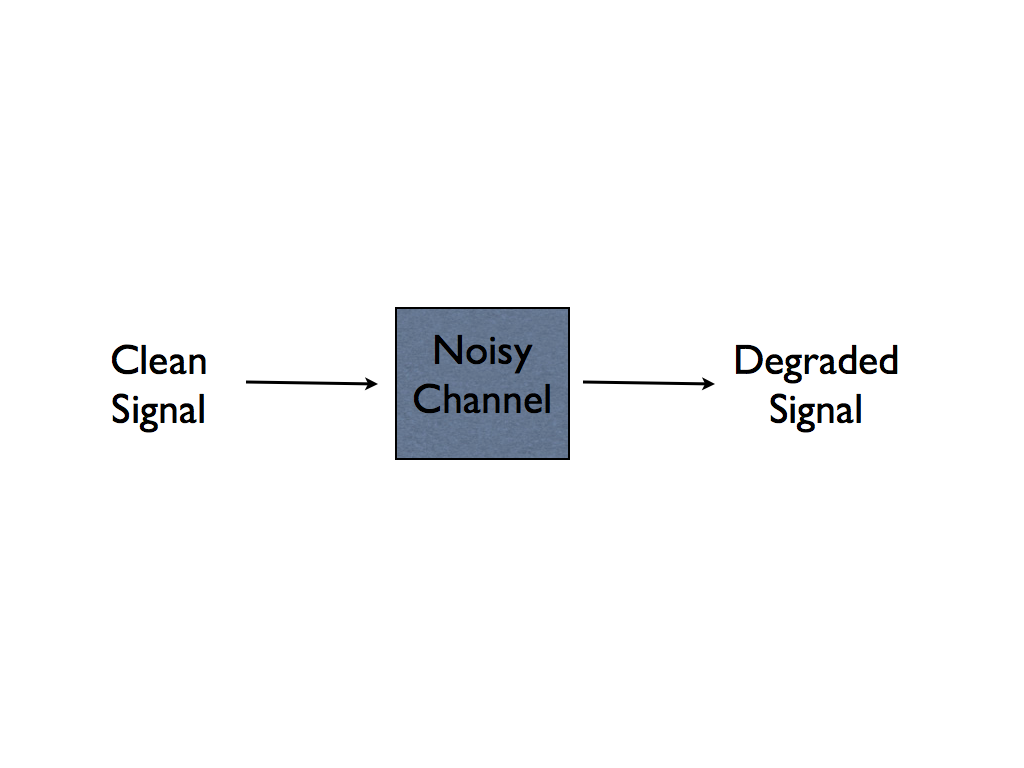
\includegraphics[clip,trim=100 300 100
    300,width=.7\textwidth]{figures/noisy_channel}
    \caption{The noisy channel model.}
    \label{noisy:channel}
\end{figure}

%The task of the listener at the far end of the noisy channel provided by the telephone is to successfully guess what the speaker actually said.  Fortunately, after a bit of experience, we become accustomed to the effects of the noisy channel, and get better at interpreting telephone speech. We call this knowledge about the channel the \keyword{channel model}: it describes the way in which the channel degrades the input speech.  Unfortunately, on its own, the degraded signal passed by the noisy channel may not be enough to reliably recover the original message. Fortunately, however, we have additional information, because we know something about the kinds of messages that we expect to hear. For telephone speech, we know, for example, that the strongest harmonics of the signal will be simple multiples of the missing fundamental frequency, which is why we are able to reconstruct the fundamental frequency even though it is not really transmitted. This knowledge about which messages are likely can be referred to as the \keyword{message model}. Taken together, the channel model and the message model can be used in a process that consumes the degraded form of the input message and produces a well-informed best guess about the original clean message.

Reviewing and formalizing our spell-checking example from \chapref{ch:writers-aids},  imagine you get an
email inviting you to a birthday party for \exword{Dsvid}.  Think of the
original clean signal as being what the user meant to type and the
degraded signal as what the users fingers actually did type.  It is
easy to tell that the clean signal must have been \exsent{David}, and that the error is a key-for-key substitution of \exword{s}
for \exword{a}, which are adjacent on a common keyboard layout. Here, the channel model says that substitutions of adjacent
keys are common, and the message model says that \exsent{David} is a
more plausible name for the mutual friend than \exsent{Dsvid}. 

We can turn the noisy channel model into math by writing

\begin{equation}
	\hat{y} = \argmax_y P(y)P(x|y)
\end{equation}
where \(x\) is the observed output of the channel (that is, the
degraded message) and \(y\) is the hypothesized clean message.  The notation \(
\argmax_y P(y)P(x|y) \) is a mathematician's way of saying ``search for
the \(y\) that gives the highest value for the probability expression
\(P(y)P(x|y)\)''. \(\hat{y}\) is therefore the system's best guess at
what the original message must have been. The message model is
expressed as \(P(y)\), which is the probability that the writer will
have intended a particular word $y$. The message model tells us that \exsent{Dsvid}
is an unlikely intended message, \exsent{David} is a likely message, and \exsent{Sara} is also a likely message, because that's also a common name.

\(P(x|y)\) is the channel model:  It tells us the probability of  receiving the degraded signal $x$ given the intended clean message $y$.  The channel model tells us that the probability of receiving the degraded message \exword{Dsvid} given the intended clean message \exword{David} is quite high (the edit distance between them is 1, and \exword{s} is even a particularly likely substitution for \exword{a} on a standard keyboard, since they are adjacent).  The channel model also tells us that the probability of receiving the degraded message \exword{Sara} given the intended message \exword{David} is quite low -- how could someone mistype \exword{David} as \exword{Sara} when they only share one letter? 

Putting together the message model and the channel model, we are looking for the $y$ that gives the highest value for $P(y) P(x | y)$.  Our degraded signal is \exword{Dsvid} and we are looking for the clean message that this signal represents.  Let's consider three candidates for the intended clean message $y$:  \exword{Dsvid, David,} and \exword{Sara}.

\begin{itemize}

\item P(\exword{Dsvid}) is \emph{low}, because \exsent{Dsvid} is not a name; P(\exword{Dsvid} $|$ \exword{Dsvid}) is \emph{high}, because if someone did for some reason mean to say \exword{Dsvid}, it is likely that they would have typed \exword{Dsvid}.

\item P(\exword{Sara}) is \emph{high}, because it's a common name; P(\exword{Dsvid} $|$ \exword{Sara}) is \emph{low}, because if someone meant to say \exword{Sara}, it's very unlikely that they would have typed \exword{Dsvid}.

\item P(\exword{David}) is \emph{high}, because it's a common name; P(\exword{Dsvid} $|$ \exword{David}) is \emph{high}, because if someone meant to say \exword{David}, it's quite likely that they would have typed \exword{Dsvid}. 

\end{itemize}

The $y$ that gives the highest value for  $P(y) P(x | y)$, combining the message model and the channel model, is thus of course \exword{David}.


At the end of the chapter, in the exercises, there are a couple of rather more exotic examples of
the noisy channel model, including part-of-speech tagging and cryptography. If you want to stretch your mind, do those exercises!
After that, there is a risk that you will start seeing the noisy channel model everywhere.

You may already be able to see why this discussion belongs in a chapter about translation. In 1949, the mathematician and information theorist Warren \citet{Weaver:1949} put it this way:

\begin{quote}
  It is very tempting to say that a book written in Chinese is simply
  a book written in English which was coded into the ``Chinese code.''
  If we have useful methods for solving almost any cryptographic
  problem, may it not be that with proper interpretation we already
  have useful methods for translation? \citep[22]{Weaver:1949}
\end{quote}

Statistical machine translation technology builds on this appealing
idea.  If we imagine that we have a
message in a foreign language  \(f\) that we would prefer to read in English
\(e\), we can factor the task into three parts:

\begin{enumerate} 
	\item Estimating a \keyword{translation model} $P(f$|$e)$.
	\item Estimating a  \keyword{language model} $P(e)$.
	\item Maximizing the product $P(e) P(f|e)$ and returning the resulting English. This process is usually called \keyword{decoding} by analogy with the cryptography example above.
\end{enumerate}



The translation model tells us the probability that a given English message $e$ could generate the received foreign message $f$.  The translation model is built on an aligned parallel corpus.  For each word/phrase in $f$, one could ask how often in the parallel corpus $f$ aligns to each word/phrase in $e$. We might also make use of a \keyword{distortion model} reflecting the probability of various reorderings of words between the foreign and English messages (or we could use some human-written transfer rules).  The translation model tells us how \keyword{faithful} the target text is to the source text; it tells us, for example, that French \exsent{le gouvernement suisse} is  very likely  given the intended English message \exsent{the Swiss government}.


The language model could be built with $n$-grams (rating the probability of a string based on the probability of the $n$-grams within it)  or it could use fancier techniques.   The main intuition is that the language model tells us the probability of a string based on its similarity to attested strings in a monolingual corpus.   The language model tells us how \keyword{fluent} the target text is as English; it tells us, for example, that \exsent{the Swiss government} is very likely English, while \exsent{the government Swiss} is less likely.


This decomposition gives rise to a nice division of labor.  Imagine
that we are trying to translate the Latin phrase \exsent{summa cum
  laude} into English, and that the system is considering three
possible candidates.
	(This example is adapted from a lecture slide by Jason Eisner.)
	
	

\ea \ea \label{latin:topmost} topmost with praise
    \ex \label{latin:cheese} cheese and crackers
	\ex  \label{latin:distinction} with highest distinction
\z 
\z 

Just as in the case of \exword{Dsvid, Sara,} and \exword{David}, we want to choose the clean intended message $y$ that gives the highest value according to the message model (language model) $P(y)$, and the channel model (translation model) $P(x | y)$.  The degraded Latin signal $x$ is \exsent{summa cum laude}, and we are evaluating three candidates for the clean intended English message $y$.

\begin{itemize}

\item P(\exword{topmost with praise}) is \emph{low}, because it's scarcely attested in English corpora; P(\exword{topmost with praise} $|$ \exword{summa cum laude}) is \emph{high}, because if someone did for some reason mean to say \exword{topmost with praise} in Latin, it is likely that they would have said \exword{summa cum laude} -- as we can infer from a translation model showing, for example, that \exword{laude} and \exword{praise} often occur in translation-equivalent Latin/English sentence pairs.

\item P(\exword{cheese and crackers}) is \emph{high}, because it's a common trigram of English; P(\exword{summa cum laude} $|$ \exword{cheese and crackers}) is \emph{low}, because if someone meant to say \exword{cheese and crackers} in Latin, it's very unlikely that they would have said \exword{summa cum laude} -- as we can infer from a translation model showing that \exword{laude} never occurs in a translation-equivalent sentence pair with \exword{cheese} or \exword{crackers}.

\item P(\exword{with highest distinction}) is \emph{high}, because it's a fairly common phrase in a monolingual English corpus; P(\exword{summa cum laude} $|$ \exword{with highest distinction}) is \emph{high}, because if someone meant to say \exword{with highest distinction} in Latin, it's quite likely -- according to translation models showing us which words tend to co-occur in translation-equivalent sentence pairs -- that they would have said \exsent{summa cum laude}. 

\end{itemize}

The $y$ that gives the highest value for  $P(y) P(x | y)$, combining the language model and the translation model, is thus \exword{with highest distinction}.

How do we choose all the candidates for $y$ to be scored against the translation model and the language model?  One common technique is to use \keyword{beam search}, a way of exploring the most promising candidates.   We build up our translation $y$ word by word using what we've learned from our automated word and phrase alignments (plus perhaps a distortion model or a series of transfer rules), and at each point we consider multiple different options for that word.  Beam search means that at each step, we store a fixed number of the most promising candidates for $y$ according to both the translation model and the language model.  At the end (when every word of the source text has been translated), we have a fixed number of good candidates for $y$ from which to choose the best one.  

In sum,  statistical machine translation constitutes yet another application of the powerful noisy channel model. By building the translation model and the language model separately, only the translation model actually needs parallel text; the language model can be built from 
 monolingual text, which can be found in greater volume.

\subsection{Neural machine translation}

Since the 2010s, machine translation has advanced using neural networks, trained by trial and error to map an input (a source sentence) to an output (a target sentence).  To translate French to English, we take a series of French/English pairs, like \exsent{Elle est am\'ericaine /END She is American /END}.  (The /END token marks the end of the sentence.)  We train the model to read in the French input \exsent{Elle est am\'ericaine /END} and output the correct translation, \exsent{She is American /END}.  The part of the network that reads in the French input is called the \exsent{encoder}, and the part that outputs the English translation is called the \exsent{decoder} (\figref{neuralmt}).


\begin{figure}
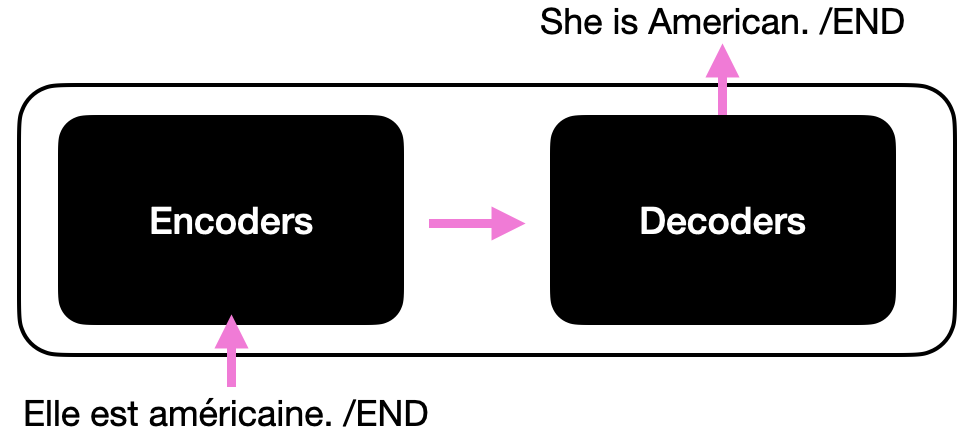
\includegraphics[width=.8\textwidth]{figures/neuralmt-fig}
\caption{Inspired by \citet{Alammar:2018}.}
\label{neuralmt}
\end{figure}


How does this work?  First, recalling the vector representations of words introduced in \chapref{ch:textasdata}, we map each French word to a number.  We do this because neural networks manipulate numbers, not strings of characters, and can use numbers to capture meaningful relationships between words.   Commonly, each word in the source vocabulary is given a unique ID number, sorted alphabetically or by frequency: Perhaps \exword{Elle} is word number 2483, \exword{est} is word 2891, \exword{am\'ericaine} is word 1322) and so on; the punctuation and the word \exword{/END} token will also have ID numbers (here, 4 and 2 -- low numbers because these special tokens will occur at the beginning of the alphabet as well as the beginning of a vocabulary sorted by frequency).  Then a source-language sentence (\exsent{Elle est am\'ericaine}) is mapped to a vector providing the IDs of its words in order.  The vector may be \keyword{padded} with 0s so that all input vectors come out to a standard length; here, it is padded to a length of seven words. 

\ea \label{encoder} \gll Elle est am\'ericaine . /END (padding) (padding) (padding) \\
     [2483, 2891, 1322,  4, 2, 0, 0, 0] \\
        \glt{}
        \z 


The target sentence is also represented as a vector, this time using a dictionary of numeral IDs for English words, also padded with 0s to a standard length.  For example, perhaps \exword{She} is word 8912.

\ea \label{decoder} \gll She is American . /END (padding) (padding) (padding) \\
     [8912, 6585, 1901,  4, 2, 0, 0, 0] \\
        \glt{}
\z 

Now comes the neural network -- a machine learning technique that takes inputs and tries to predict the correct outputs.  The input French sentence, represented as \REF{encoder}, is fed to a layer of \keyword{nodes}.  Each node represents a function involving some multiplication and addition, specified using values called \keyword{weights}, which operates on the vectors that we feed to it.  After all this multiplication and addition, we have a new vector that represent the French sentence.  Then we can feed this new vector to another layer of nodes, where we do some more multiplication and addition using a new round of weights.  Eventually, the final layer takes in a vector (generated by the previous layer), does some multiplication and addition with a final layer of weights, and outputs a probability function that it uses to decide what it considers to be the most probable English translation -- our output.  Namely, for each word in the target translation, the model outputs a vector of all the words in the target vocabulary such that each one is associated with its probability of being the correct output. Ideally, it should give the highest probability to the correct word \exword{She} (word 8912), but perhaps instead it has given the highest probability to the word \exword{the} (word 9901).
Then our system goes on to predict the next word of the target, considering the entire input sentence along with the output that it has generated so far.  When it predicts the \exword{/END} token, it stops predicting words, pads the rest of the output with zeroes, and returns its translation.

While training the model to predict the second target word (\exword{is}), it can be helpful to let the model see the correct first word of the target (\exword{she}) rather than the one it has predicted (perhaps the erroneous \exword{the}); that way, it learns to predict the second word as if it had gotten the first word right, rather than swerving off-course by trying to complete a sentence that has already gone astray.   This technique, letting the system see the correct target word \exword{w1} when trying to predict \exword{w2}, is called \keyword{teacher forcing} and resembles how human teachers may scaffold students working through a multi-step problem.


The power of the neural network comes from the process by which we learn the best weights for each layer.  We choose some random weights to start, and then use \keyword{error-driven learning} to learn the best ones through trial and error.  First, we do a \keyword{forward pass} through the network, inputting a French sentence to get an English output.  The first time we pass a French sentence like \exsent{Elle est am\'ericaine /END} through the network, it might output a terrible English translation like \exsent{the the the /END}.  
Each time the model produces an output, it checks how well it did by calculating what probability it assigns to the correct output (\exsent{She is American /END}).  Here, the network gave a higher probability to \exsent{the the the /END} than to the desired output \exsent{She is American /END}, so the network realizes that it has made an error.   Now it needs to update its weights to give a higher probability to the correct translation \exsent{She is American /END}. 

So the next step is \keyword{back-propagation}.  We do a \keyword{backward pass} through the network, starting with the erroneous output, and walking back through the network to adjust all the weights that gave rise to this error.  Layer by layer, we go look at each node,  figure out how much that particular node contributed to this error, and update the weight of each node to reduce the error.  (This process is called \keyword{gradient descent} -- we use the idea of gradients from calculus to figure out how much each node caused the error, and we update the node's weight so that the error descends downward.)   We might use several thousand training examples, and we might pass all of those examples through the network multiple times.  (Each pass through our training data is called an \keyword{epoch}.)   Each time, we recalibrate all the nodes to reduce the error.    

Eventually, we end up with a system that has ``learned'' to map French sentences to English ones.  Once trained, the network can be evaluated using test data in the form of  French/English pairs that it hasn't seen before; and ultimately, it can be turned loose on French sentences that don't appear in any parallel corpus at all.  


%As we've already seen elsewhere in this book, the neural networks underlying neural machine translation -- just like the noisy channel model underlying statistical machine translation -- constitute an extremely powerful idea with many applications beyond translation or language.  We can just as easily train a neural network that maps houses (represented as vectors, reflecting attributes like square footage and neighborhood) to their prices, or a neural network that maps images of handwritten digits (represented as a vector of pixels) to the Unicode 0--9 digit that each image represents.  To build a neural network, all we need is some training data consisting of inputs paired with their correct outputs: some houses and their prices; some images of handwritten digits and their labels; some correctly translated French-English pairs.

%Of course, we also need a conceptual reason  that these outputs should indeed be predictable from our inputs.   Even if you can find training data, there is no sense in building a neural network that would map the weight and heart rate of a newborn baby to the field that they study in college, for example, because there is no reason to think that a baby's birth statistics are at all related to their academic interests.   But we are quite justified in thinking that a house's price can be predicted from its square footage and location, and in thinking that an English translation can be predicted from a French source sentence.  We also need to think about where our training data comes from, who created it, what limitations it may have, and where it may reflect various types of bias.   Even if neural networks seem shockingly intelligent, we can never forget our own humanistic  capacity for critical thinking.

%These examples already illustrate that neural networks come in many flavors.  Some neural networks predict continuous outputs (mapping houses to their  price, in dollars), which is called \keyword{regression}.  Others map the input to one of several predefined bins (mapping handwritten digits to 0, 1, 2, 3, 4, 5, 6, 7, 8, or 9; mapping emails to \exword{ham} or \exword{spam}), called \keyword{classification}.  We may use classification as a first step in machine translation, if we are given a string of text and have to figure out what language it's in before we can translate it.  This type of classification is called \keyword{language identification}: our input is a sentence, and our output is the language label (Yoruba, Dutch, French, \ldots). 

In the case of machine translation, we map a sequence of source words to another sequence of target words, which is called a \keyword{sequence-to-sequence} problem.  Sequence-to-sequence problems are harder than regression or classification because instead of just outputting a number or a classification label, we have to output an open-ended sequence of words.

Word sequences (sentences) are interesting because each word in a sentence is more or less related to other words -- within the source sentence, within the target sentence, and across those two sentences.  In the French source sentence \exsent{Elle est am\'ericaine}, the third-person-singular verb \exword{est} agrees in number with the singular pronoun \exword{Elle}, and feminine adjective \exword{am\'ericane} agrees with \exword{Elle} in gender.  In the English target sentence, \exword{is} agrees with \exword{She} in number.  Moreover, coming back to the idea of word alignment, the French words are related to the English words: \exword{Elle} aligns with \exword{She}, \exword{est} aligns with \exword{is}, and \exword{am\'ericane} aligns with \exword{American}.  The sequence-to-sequence neural network needs a way of capturing all of these relationships.  

One powerful way of doing this uses an idea called \keyword{attention} \citep{Vaswani-etal:2017}. We train a layer of weights in the network to decide, for each word in the output, how much \keyword{attention} it should pay to each word in the input -- how much that input word should affect the choice of the right output word.  For example, as we try to translate \exword{She}, the attention mechanism tells us to pay the most attention (give the most weight) to \exword{Elle}.  Thus, as the attention mechanism is trained in tandem with the rest of the network,  it ends up discovering word alignments in a bottom-up manner.   This mechanism is called \keyword{encoder-decoder attention} because it tells us, for each word to be decoded in the output, how much it depends on each encoded word in the input.     We can visualize encoder-decoder attention in a two-dimensional diagram (\figref{attn-fig}) with the source sentence on one axis and the target output on the other; a lighter-colored square means that the decoder was trained to pay attention to the corresponding word in the encoder. 

\begin{figure}
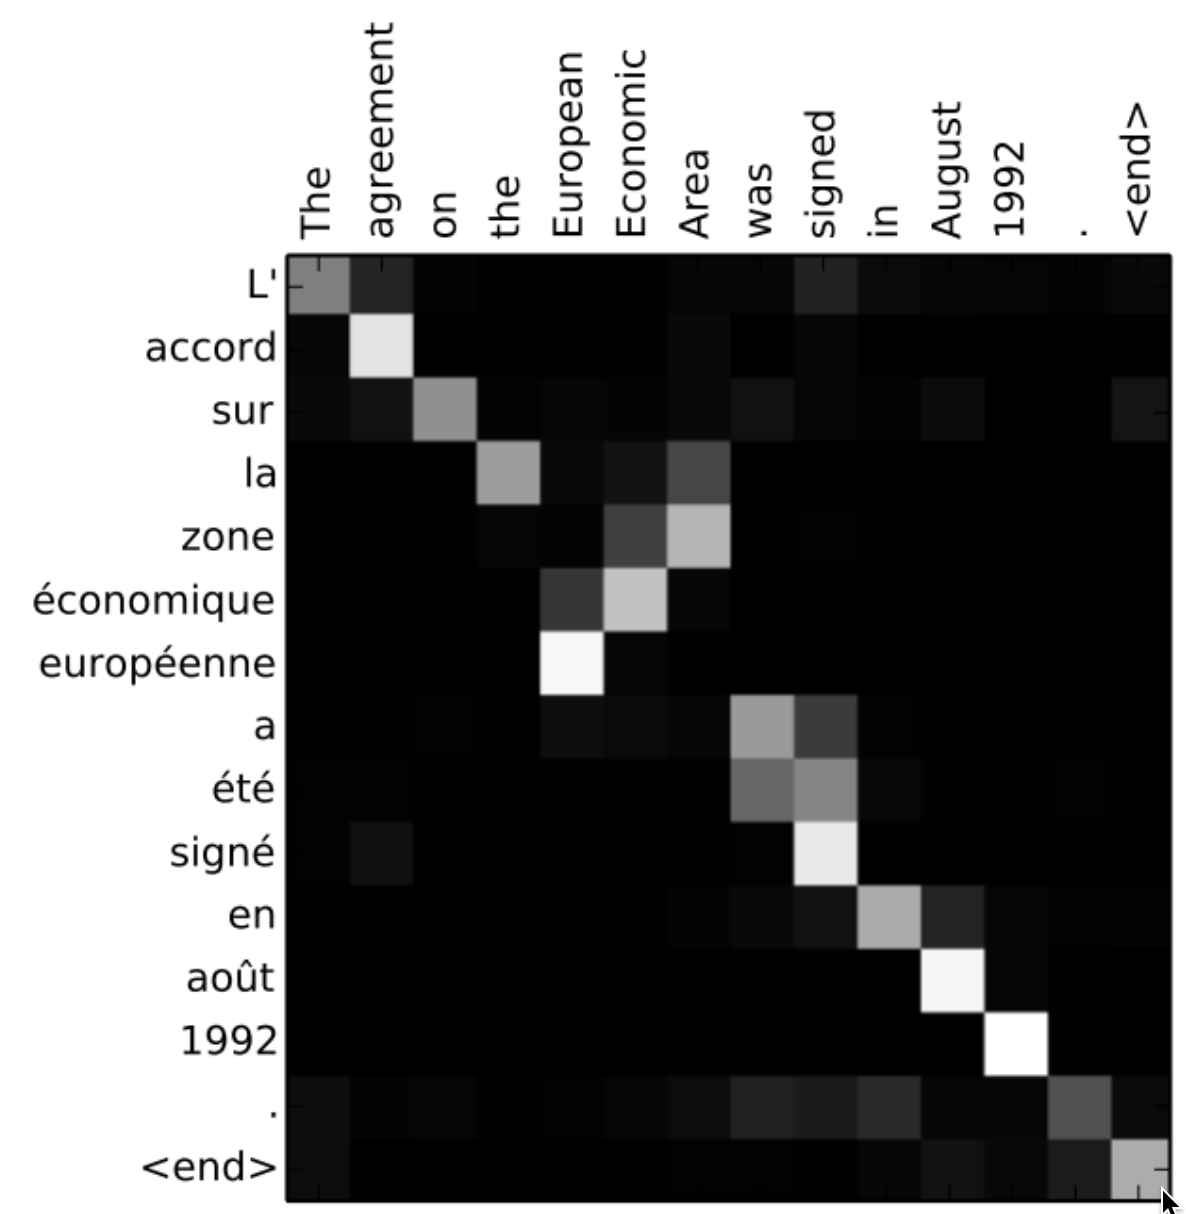
\includegraphics[width=.7\textwidth]{figures/attn-fig}
\caption{Reproduced from \citet{Bahdanau-etal:2015}. \small{The code that generates this figure) is public -- copyright  2014, Machine Learning Lab (LISA) at University of Montr\'eal -- and shareable; see \url{https://github.com/lisa-groundhog/GroundHog}.}}
\label{attn-fig}
\end{figure}


We can also use an attention mechanism to relate each input word to other input words, or each output word to other output words: As we try to translate \exword{is}, the attention mechanism tells us to pay attention to the previously generated output word \exword{She}, since \exword{is} agrees in number with \exword{She}.  This mechanism is called \keyword{self-attention} because each word in the output is associated with other words within itself, rather than being associated with a word in the input.

Attention mechanisms underlie the most successful neural machine translation systems in use today, such as Google Translate.  Beyond their empirical effectiveness, attention mechanisms have also been argued to offer the conceptual advantage that they help shed some light onto the otherwise opaque knowledge represented by the neural network.    How do we understand the meaning of a trained weight vector like [0.02, -9.25, 10.2, \ldots]?  Attention visualizations such as those shown in Figure \ref{attn-fig} may help us  \keyword{interpret} or \keyword{explain} the network's behavior.

The mathematical implementation of all these ideas lies beyond the scope of a general-interest textbook, but the take-home points are that:

\begin{itemize}

\item Modern machine translation uses sequence-to-sequence neural networks.  The network is trained on a parallel corpus to predict the right target-language output given a source-language input.

\item Neural networks learn by trial and error.  The network tries to predict an output, checks where it went wrong, and then updates weights to do better next time.  Over thousands of iterations, the network can become very successful.

\item The idea of word alignment from statistical machine translation re-emerges in a modified form as attention -- a mathematical way of associating each word with the other words most related to it, both within a sentence and across source-target pairs.

\end{itemize}

% training - you could try to maximize BLEU score, but that is NOT usually what people do; instead they try to give the highest probability to the actual correct output sentence, word by word


\subsection{Evaluation}

Having built a machine translation system, it is useful to be able to evaluate how well it is doing.  
One popular automatic evaluation metric proposed by \citet{Papineni-etal:2002} is known as \keyword{BLEU} (Bilingual Evaluation Understudy), parallel to the concept of \keyword{precision} discussed in \chapref{ch:text-classification}.  We compare a machine-generated \keyword{candidate translation} to one or more human-written \keyword{reference translations}.  BLEU can be calculated as the number of words in the candidate translation (C) that also appear in some  reference translation (R), divided by the length of the candidate translation. 
\begin{equation}
\mbox{BLEU score} = \frac{\mbox{number of words in C that also appear in R}}{\mbox{total number of words in C}}
\end{equation}

  If our candidate translation is \exsent{I love running} and the reference translation is \exsent{I love to run}, then our BLEU score is 2/3: Two words in the candidate translation (\exword{I, love}) also appear in the reference translation (so 2 is the numerator), and the candidate translation is three words long (so 3 is the denominator). We can also compute fancier versions of BLEU which look at larger $n$-grams rather than just single words (unigrams). 

If our candidate translation was just \exsent{love}, it would get a perfect BLEU score of 1: One word in the candidate translation also appears in a reference translation (thus, the numerator is 1), and the candidate translation is one word long (thus, the denominator is 1).  That's why the calculation of BLEU may also  use  a \keyword{brevity penalty} to down-grade candidate translations that are too short.


Of course, \exsent{I love running} means basically the same thing as \exsent{I love to run}, so maybe our candidate translation should really get a higher score than just 2/3.  (Indeed, if we had more than one human-written reference translation to compare against, the BLEU score would probably go up.) This example illustrates why it can be difficult to evaluate machine translation automatically.  We want to ask whether the candidate translation captures the meaning of the source sentence, but without any way of representing meaning, we have to use  imperfect cues like BLEU to evaluate translations.



\section{Consequences}

For many years, machine translation was considered the hardest problem in NLP.  During the Cold War, a report by the United States National Academy of Sciences  \citep{alpac:1966} argued that machine translation (namely, Russian-to-English translations of scientific research) was of such poor quality that it was not a good use of government resources, and that money would be spent more efficiently on human translators and tools, such as scientific glossaries, to help them.  That pessimistic ALPAC report is often cited as the reason that machine translation attracted scant funding for decades.  But today, the authors of that report might be surprised that machine translation (for some language pairs) is astonishingly good and gets better every day. 

Perhaps machine translation seemed difficult in part because human translation is difficult. A human translator must be highly literate in two languages, which requires years of schooling, and many of us do not have that expertise.  But in reality, machine learning has progressed in part because it has a ``right answer'' in the form of a parallel corpus.  Whenever we can find a lot of training data mapping inputs to output  ``right answers'', the power of machine learning can make a lot of progress in learning that mapping.

But machine translation still faces challenges.  We've already seen that translation sometimes requires cultural knowledge or knowledge of the world that is not represented in the source text (what gender should \exword{my neighbor} be given in French?).  Sometimes, a machine translation system may use statistical biases to choose gendered translations, as in this English-to-Spanish example from \citet{Stanovsky-etal:2019}.  


\ea English original \\
	The doctor asked the nurse to help her.

\ex Spanish machine translation \\
    \gll El doctor le pidi\'o a la enfermera que le ayudara. \\
    the.\textsc{masc} doctor.\textsc{masc} 3\textsc{sg} asked to the.\textsc{fem} nurse.\textsc{fem} that 3\textsc{sg} would-help \\
    \glt{`The (male) doctor asked the (female) nurse to help.'}

\z 

The English original indicates a female doctor through the pronoun \exword{her} later in the sentence, and doesn't specify the gender of the nurse.  But the Spanish translation defaults to the masculine form of the word for `doctor' and the feminine form of the word for `nurse', presumably because those forms are more common in its training data, thus perpetuating professional gender stereotypes.

Machine translation also struggles with low-resource languages, and has a hard time  translating text from a domain different from its training data (a system trained on the Bible may struggle to translate tweets).  It can be hard to identify or translate named entities: In a sentence like \exsent{Holly loves swimming}, how can we recognize \exword{Holly} as a name rather than a plant?  It is also hard to deal with new words that weren't present in the training data: How will your system translate \exword{pantsgate} (a pants-related scandal, using the \exword{-gate} suffix popularized by the Watergate political scandal) if it's never seen this word before?  And how should it be translated when this \exword{-gate} suffix evokes rich cultural knowledge, perhaps opaque to foreigners, of the Watergate scandal in American history?  For literary works, one might also worry that a machine translation would miss subtleties of connotation, double meanings, and rhyme. 

We may also be curious what ideas from linguistics emerge (or don't emerge) bottom-up in the representations learned by neural networks.  Does the network encode any information that linguists would recognize as part-of-speech tags, syntax, or semantics?  At the time of writing, the sentence \exsent{At Cannery Row, people can tuna} is still mishandled by English-to-French Google Translate, which translates \exword{can} as the modal \exword{pouvoir} `to be able to' rather than the comparatively rare verb `to put into a can' -- so the system struggles with linguistic notions such as sense disambiguation (which sense of \exword{can} should be used?) and syntax (what's the verb in this sentence?).

Returning to our recurring question about whether humans and computers compete or complement one another, what are the consequences for human translators now that machine translation is so successful?  Human translators created the parallel corpora used to train machine translation systems.  But do machine translation enterprises adequately credit and compensate them for this work?  And will human translators eventually be replaced by the machine translation systems that their data helped to build?  

A pessimist would say that a few human translators will still be needed in high-stakes contexts, but that many others will lose their jobs.  An optimist would say  that human translators will work alongside machine translation systems, each complementing one another's strengths, to build a more interconnected global society.  The machine translation system may be used to generate draft translations;  the human can post-edit and finalize, prevent cross-cultural misunderstandings, and track down world knowledge like the locations of prisoner-of-war camps and the gender of people's neighbors.  



Finally, what are the consequences of machine translation for the people whose  writings are translated?  Does widely available machine translation reduce the need to learn a second language (in a classroom, or with CALL tools as discussed in \chapref{ch:call})?  Does it allow people to communicate more easily around the globe? 

Or could it cause misunderstandings?  In 2017\footnote{\exword{The Guardian}, ``Facebook translates `good morning' into `attack them', leading to arrest,'' by as reported by Alex Hern, 24 October 2017.}, a Palestinian construction worker Facebook-posted a photo of himself with a bulldozer, and a caption that said  \exword{Good morning} in Palestinian Arabic.  Machine translation systems can struggle with  Arabic because most formal writing uses Modern Standard Arabic whereas speech and social media posts use regional varieties that are not mutually intelligible (a situation known as \keyword{diglossia}).  So Facebook's system translated \exword{Good morning} as `Attack them' -- which, combined with the image of the bulldozer, was interpreted by Israeli police as a violent threat. The construction worker was arrested and questioned for hours.

Unfolding within the larger Arab-Israeli conflict, this unfortunate event was specifically triggered because Facebook's translation system not only failed to translate Palestinian Arabic, but also failed to anticipate how the technology would be used, and failed to signal its fallibility to the police who wrongly relied on its output.  Returning to the theme of how technology should be used ethically, one might conclude that automated systems should transparently flag low-confidence output, and that even high-confidence output should be checked by a human before it is used to arrest someone.


%  BUT, what are its challenges?? -- out-of-domain data, low-resources conditions, low-resource languages maybe
% human trust appropriate????

%\item how INTERPRETABLE are these systems?  how do we understand WHY it gives the output that it gives?

% Named Entities - when should you leave a name alone, how do you identify a name as such, should you translate the name `Holly' into another language?  Names aren't always capitalized btw (back to Writing Systems)
% what do you do with unknown words?  named entities? break them into subwords?  look them up in a dictionary?

% Cannery Row example
% how much top-down insight from linguistics will be helpful?

% consequences for human translators?



% then close with a discussion of why MT is maybe NOT AS HARD AS it seemed!!!.
% but what is the hardest part about it?
% ethics - story about the guy who was arrested in Israel.
% complementarian approach for humans and computers maybe.




%Translators entering the professional market will need to become  expert on how to use translation memories, electronic dictionaries  and other computer-based tools. They may rely on automatic  translation to provide first drafts of their work, but will probably  need to create the final drafts themselves, and the need for expert  human judgement will certainly not go away. In part, this is because  users of commercial translation need documents that they can rely on, so they want a responsible human being to vouch for the accuracy and  appropriateness of the final result.  Specialist commercial  translators will certainly continue to be in demand for the  foreseeable future: there is no need to worry about the risk of being  replaced by a computer. As in most other workplaces, you have to be  comfortable {\bf using} technology, and you should expect to have to  keep learning new things as the technology changes and offers you new  ways of doing your job efficiently.

%The range of languages for which free web-based translation is available will continue to grow, because the statistical techniques that are used are very general, and do not require programmers to have detailed knowledge of the languages they are working with.  In principle, given a parallel corpus, a reasonable system can be created very rapidly.  A possible example of this was seen in June 2009, when Google responded to a political crisis in Iran by rolling out a data-driven translation system for Persian.  It appears that this system was created in response to an immediate need, because the quality of the English translations from Persian did not match up to the results from Google's system for Arabic, which used essentially the same technology, but had been tuned and tested over a much longer period.  


%Literary and historical translators could be unaffected by all this, although some of them will probably benefit from tools for digital scholarship such as those offered by the Perseus Project.  These allow scholars to compare different versions of text, follow cross-references, seek out previous works that might have inspired the current work, and so on. For example, a scholar working on a Roman cookbook might want to check up on all uses of the word \exsent{callosiores} in cooking-related Latin, to see how often it seems to mean `harder' and how often it means `al dente'.

%Many potential users want to use automatic translation as a tool for gathering a broader range of information than they otherwise could.  Marketers who already do the kind of opinion mining mentioned in chapter~\ref{ch:text-classification} will also want to collect  opinions from their non-English-speaking customers. This is much the same as what we did to decode the German cell-phone review.

\begin{tblsfilledsymbol}{Checklist}{test}

\begin{itemize}
\item Give examples of various translations needs, some which require human expertise, and some which  can be easily automated.
\item Draw and explain the translation triangle. You should be able to use the idea of more abstract and less abstract representations, and explain why the distance between the source language and the target language narrows as we move up the triangle towards more abstract representations.
\item Identify several typological differences between languages and explain their significance for machine translation.
\item Give examples of cases where a translator needs knowledge beyond the source text in order to translate.
\item Explain the idea of word alignment. You should be able to take a pair of sentences and draw lines to indicate which words in the source language are aligned with which words in the target language.  
\item Explain the noisy channel model and how it can be applied to different types of tasks, including machine translation.
\item Compare and contrast statistical and neural machine translation.
\item Define encoder-decoder attention and self-attention.
\item Calculate the BLEU score of a candidate translation with respect to a reference translation.  Explain how BLEU echoes the idea of precision from \chapref{ch:searching}.
\item  Explain why machine translation is perhaps easier than it first appeared, and what challenges it still faces.
\end{itemize}
\end{tblsfilledsymbol}


\begin{tblsfilledsymbol}{Exercises}{pencil}
    
\begin{enumerate}

\item  Please return to the bulleted list of possible translation needs in Section \ref{translateneeds}.  Discuss with a partner whether you would use machine translation or a human translator in each situation.  If you would hire a human, please discuss what qualifications you would want them to have.


\item  Using the example from \citet{Jurafsky.Martin-09}, discuss how you would translate \exsent{The Lord is my shepherd} (Psalm 23) into a language spoken in a culture without shepherds or sheep.


\item Please choose a non-English language that you are familiar with, and observe at least one distinction (such as formality, number, gender, evidentiality, definiteness, or tense) that is marked in this language but not in English or vice versa.  

\begin{itemize}
    \item Please provide a specific example of a sentence in this language (glossed word-by-word and translated into English) showing that this distinction is marked in only one of the two languages.
    \item Next, please choose your favorite machine translation system, and discuss how this sentence is automatically translated in both directions.

\end{itemize}

\item Find a native speaker of a language other than yours (and other
	 than English), and sit down with them with a short passage of text
	 in their native language.  Discuss what problems there are in
	 translating from their language into English (or into your own
	 native language).  Which kinds of sentences/constructions are fairly
	 easy to translate?  Which ones border on impossible?


\item   Explore the World Atlas of Language Structures.\footnote{\url{www.wals.info}, accessed 2024-04-26.} Look at some of the ways that languages vary in terms of syntax and semantics, and articulate the consequences for machine translation systems.

\item   Explore the Endangered Languages Project.\footnote{\url{www.endangeredlanguages.com/}, accessed 2024-04-26} Choose an endangered language to explore.   Does this language have a writing system? Is this language available on Google Translate?  Can you find any parallel corpora online\footnote{\url{https://opus.nlpl.eu}, accessed 2024-05-23.} that use this language?  

	\item The three procedural languages of the European Union are English, French and German. There are twenty-one other official languages, making 
a total of twenty-four.
	You want to make sure that it is possible to translate from any of these languages to any other. Twenty-four languages means 276 unique language pairs (mathematically, twenty-four choose two); if each pair needs a different person to translate in each direction (e.g., Slovenian to Greek, Greek to Slovenian), then we would need 552 different translators. But how many translators  do you need if you adopt a policy that all documents will be first be translated 
	from the source language into English, French or German, then translated back out into the target language? How many would you need if you managed to agree that there should be just one procedural language (for example, German) and that all translations would either begin, end or pass through German? 
	



	\item Try out Google Translate using English and another language that you know.
	 \begin{enumerate}

	 \item Choose three sentences as a test suite.  Try sentences that include information that is marked grammatically in one language but not another (for example, gender on nouns is marked in French but not English; tense on verbs is marked in English but not Chinese).  You could also try \exsent{At Cannery Row, people can tuna}, or a sentence including a word that is ambiguous between a proper name and a noun (\exsent{I like Holly}).
    \item     Try translating these sentences from English into this target language.  Using your knowledge of the target language, rate the quality of these translations.  How well does the translation handle tricky issues, such as information that is marked in one language but not another?
    \item Now ask the machine translation system to translate these sentences \emph{back to English}.  How good are these translations?  How similar are they to the original English input?
    \item  If the translation back to English matches the original English input, does this mean that the target language translation is necessarily high-quality? Why or why not?  
    \item Compare notes with classmates who tried different target languages.  Do you see evidence that some language pairs offer higher quality translation than others?
    \item Now try different types of source texts -- recipes, tweets, song lyrics, and news text.  What type of text is translated the best?
\end{enumerate}
	

\item The math for the noisy channel can also serve as
a way of working out the parts of speech mentioned in
Section~\ref{part:of:speech}. We have to imagine that speakers were
once really cooperative, and that instead of speaking normally, and
saying things like:


\ea \label{ex:part:of:speech:1}He checked out a book
  from the library.
\z 

they actually used to say:

\ea \label{ex:part:of:speech:2}He/pronoun checked/verb
                                out/adverb a/article book/noun \\
                                from/preposition the/article 
	                            library/noun ./punctuation
\z 

helpfully spelling out all the parts of speech for us. Unfortunately, people no longer speak like this, so, if we want the parts of
speech, we must guess them. We can think of
 \REF{ex:part:of:speech:2} as being \(y\) (the clean message)
and \REF{ex:part:of:speech:1} as being \(x\) (the degraded
form of the message). In other words, we are imagining that people
still really speak in a form that spells out the parts of speech, but
that everything they say is filtered through a very noisy channel that
deletes the part-of-speech tags and retains only the words. Of course,
this is not actually what is going on, but we can still go through the
steps of searching for the part-of-speech sequence that is most likely
to go with the words that we saw. 

Finish this story by designing a part-of-speech tagging model that
\begin{enumerate}
\item Uses probabilities of the form \(p(tag_2|tag_1)\) to model the chance that, for example, a noun will follow a verb.
\item Builds up the probabilities of longer series of tags by chaining together the individual probabilities  \(p(tag_2|tag_1)\)
\item Uses probabilities of the form \(p(word|tag)\) to model the chance that, for example, a randomly chosen noun will
turn out to be the word \exsent{dog} (or \exword{zebra} or \exword{axolotl})
\end{enumerate}

Test whether you fully understand your model by seeing whether you can explain to yourself  how it would give different probabilities to two different interpretations of
the sentence \exsent{He saw her duck}. 

If you can spell out the details of this model on your own, without further clues, you will have reproduced one of the better achievements of computational linguistics. If you need further hints,  \citet{Jurafsky.Martin-09} 
covers this approach to part-of-speech tagging.

\item You can also apply the noisy channel model to
cryptography. Imagine that you receive a coded message mentioning an
impending invasion of Britain by \exsent{MXOLXV FDHVDU}. As an expert
in cryptography, you know to shift each letter three letters back in
the alphabet and identify the culprit \exsent{JULIUS CAESAR}. To get from \exword{M} to \exword{J}, we look at the alphabet -- \exword{J,K,L,M} -- and rewind three letters back from \exword{M} to land on \exword{J}. 

Here
\(y\) is the original Latin name, \(x\) is the encoded message, the
channel model says to shift three letters forward, and the message
model is about a person who is a likely invasion threat. The channel is
specifically designed so that those who are in the know can undo its
corrupting effect.   

You now receive a message using the \emph{rail fence cipher}, which involves laying
out the message in the form of a rail fence, then reading it off row by row.
Here is an example of how the message \texttt{TRANSPOSITION CIPHERS ARE FUN}
would be laid out in a four-rail cipher.
\begin{verbatim}
T.....0.....N.....R.....U.
.R...P.S...O.C...E.S...F.N
..A.S...I.I...I.H...A.E...
...N.....T.....P.....R....
\end{verbatim}
In cryptography, we leave out the spaces between the words, and group the encoded message into fives, so
this message would be encoded as \texttt{TONRU RPSOC ESFNA SIIIH AENTP R}.
In order to read the message, the recipient has to know that when the message was sent, the writer used
four rails. Knowing that, it is possible to recreate the layout and read off the message, once again in the conventional
cryptographic groups of five, as 
\texttt{TRANS POSIT IONCI PHERS AREFU N}. All that remains is to regroup the letters into words, and the reader has decoded
the message.
If the reader uses three rails instead of four, this happens:
\begin{verbatim}
T...O...N...R...U...R...P.
.S.0.C.E.S.F.N.A.S.I.I.I.H
..A...E...N...T...P...R...
\end{verbatim}
and the decoded message is \texttt{TSAOO CEENS NFRNT AUSPI RIRIP H}. The fact that this is 
unrecognizable gibberish
proves that a mistake has been made somewhere.

The process for encoding is.
\begin{itemize}
\item Lay out a grid with the right number of rows. If you use four rows and your friend uses three, this is not 
going to work.
\item Start at the top of the grid, and fill in cells diagonally downwards, until you reach the
bottom row.
\item Turn around and write diagonally upwards until you get to the top.
\item Keep writing diagonally up-and-down until you run out of message text.
\item Read off the text by rows.
\end{itemize}
Consider the following rail fence message \texttt{TAEIS HRIFN ESAYE LCE}.
\begin{itemize}
\item What does the decoded version of the message say? You might have to try a few different numbers of rows.
\item How many rows are there in the rail fence that worked? 
\item In the noisy channel formulation of the rail fence, we know that the channel model is ``it was corrupted by the railfence cipher''. 
Describe the message model that you used, and how it helped you to decide whether you had solved the problem.
How would this message model need to change if there was a possibility that the sender was from a foreign country?
\end{itemize}

\item    When translating from English into the Native American language Mam
  (in Guatemala), a translator reported the following terms used among
  siblings (in phonetic transcription here):

  \begin{itemize}
  \item{} {[ntzʔica]} = `older     sibling'
  \item{} {[witzin]} = `younger     sibling'
  \end{itemize}
        
  Both words are used for males and females.

  \begin{enumerate}
        
  \item In terms of hyponymy/hypernymy, describe the relationship
    between the English word \exsent{sibling} and these words.

  \item Draw a Venn diagram showing how the English words
    \exsent{brother} and \exsent{sister} overlap with the Mam words
    {[ntzʔica]} and {[witzin]}.

          
  \item You come across the text: \exsent{Maxwell is the brother of
      Santiago}, but it gives no indication of who is older.  If you
    had to translate this into Mam and were being forced to preserve
    this age ambiguity, how would you do it?
  \end{enumerate}

\item Please list the following tasks in increasing order of difficulty for a computer, and for a human.  What can you say about the differing strengths of humans versus computers?

\begin{itemize}

\item Translating a document from French to English.

\item Playing chess.

\item Having a supportive, empathetic conversation with a friend about a problem she's been having at work.

\item Reading a social media post and deciding if the person who wrote it is morally correct or not (please see the subreddit r/AmITheAsshole for examples).

\end{itemize} 

\item Go to a multilingual website\footnote{\url{https://www.biblegateway.com/}, accessed 2024-04-18.}  and check out Genesis, Chapter 1, verses 1 and 3 (``In the beginning God created the heavens and the earth [\ldots] And God said, `Let there be light,' and there was light'') in a variety of languages.  (These verses are good because the words \exword{God, and,} and \exword{light} are repeated; we do not intend to make any religious statement by choosing this text).  See if you can align the words across different languages.

\end{enumerate}
\end{tblsfilledsymbol}


\begin{tblsfilledsymbol}{Further reading}{book}
    
The following textbooks offer valuable chapters on machine translation:

\begin{itemize}

\item Jacob Eisenstein's  textbook \citep{Eisenstein:2019}.

\item Jurafsky and Martin's regularly updated textbook \citet{Jurafsky.Martin-09}, recently updated as a draft on Jurafsky's website.

\item \mediatitle{Language Files} \citep{LanguageFiles13}.

\end{itemize}

There are also full (e-)books on the topic:

\begin{itemize}

\item Philipp Koehn's  book \textit{Neural Machine Translation}  \citep{Koehn:2020}

\item Graham Neubig's  2017 ``Neural machine translation and sequence-to-sequence models: A tutorial'' : \url{https://arxiv.org/pdf/1703.01619.pdf} \citep{Neubig:2017}

\end{itemize}

There are also some great blog posts and Python Notebooks online showing you how to build your own neural machine translation system -- just search for ``neural machine translation notebook''.

As mentioned above, \citet{Piron:1988} discusses how translation requires a lot of research into the real-world state of affairs described in the source text, and expresses a pessimistic view of machine translation.  In light of the recent advances in machine translation, to what extent are his concerns still relevant?

Jay Alammar's blog post \citep{Alammar:2018} provides illuminating illustrations of neural machine translation with attention.



The Perseus project \citep{perseus} presents beautiful web versions of
literary texts, including 13 million words of Latin and 10 million
words of Ancient Greek. These include commentary, translations and all
kinds of support for multilingual scholarship.

\citet{NordhoffKramer:2022} offer a dataset of glossed examples from lower-resourced languages, scraped from books published by Language Science Press.\footnote{\url{https://imtvault.org/}, accessed 2024-04-18.}

\end{tblsfilledsymbol}
